\documentclass[12pt,a4paper,conference]{IEEEtran}
\usepackage[utf8]{inputenc}
\usepackage[english]{babel}
\usepackage{amsmath}
\usepackage{amsfonts}
\usepackage{amssymb}
\usepackage{graphicx}
\usepackage{subcaption}

\usepackage{float}
\usepackage{fullpage}

\usepackage[hidelinks]{hyperref}

\usepackage{tikz}

\usepackage{todonotes}
\usepackage{epstopdf}
\usepackage{graphicx}
\usepackage[T1]{fontenc}


\let\ig\includegraphics
\renewcommand{\includegraphics}[2][]{ \IfFileExists{#2}{ \ig[#1]{#2} }{ 
		\IfFileExists{#2.eps}{ \ig[#1]{#2} }{ 
		\IfFileExists{#2.png}{ \ig[#1]{#2} }{ 
		\IfFileExists{#2.jpg}{ \ig[#1]{#2} }{ 
		\IfFileExists{#2.jpeg}{ \ig[#1]{#2} }{ 
		\IfFileExists{#2.gif}{ \ig[#1]{#2} }{ 
		\IfFileExists{#2.ppm}{ \ig[#1]{#2} }{ 
		\missingfigure{  \protect\detokenize{#2} was not found.} 
}}}}}}}
}

\newcommand{\missingequation}[1]{\todo[inline, color = yellow]{Missing equation: #1}}


%%
%% End of file `mypackage.sty'.

\newcommand{\cutOutWidth}{0.45 \linewidth}
\newcommand{\histogramWidth}{0.8 \linewidth}
\newcommand{\fullImageWidth}{0.8 \linewidth}


\begin{document}
\raggedbottom

\title{Visual Servoing\\ \large{ROVI - Finalproject}}
\author{Nicolaj Iversen and Lukas Schwartz}
\date{18$^{th}$ December 2015}

\maketitle

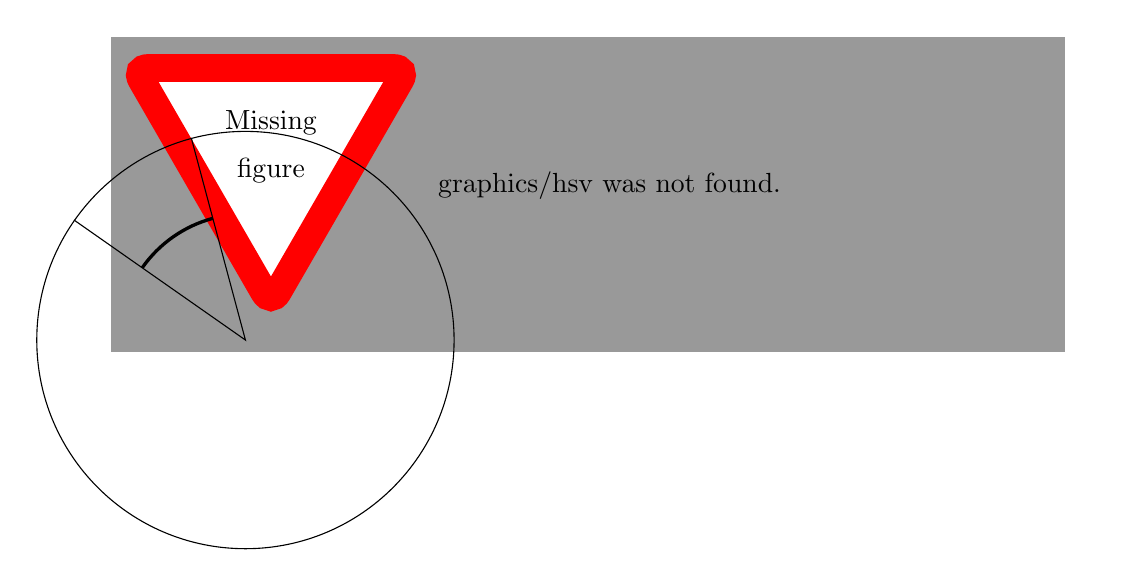
\begin{tikzpicture}
% % % % RED % % % %
% \newcommand{\MinHue}{-10} %angle
% \newcommand{\MaxHue}{20}
% \newcommand{\MinSat}{2cm} % 0 - 1 => 0 - 2.65
% % % % GREEN % % % %
\newcommand{\MinHue}{105} %angle 
\newcommand{\MaxHue}{145}
\newcommand{\MinSat}{1.6cm} % 0 - 1 => 0 - 2.65
% % % % BLUE % % % %
% \newcommand{\MinHue}{220} %angle
% \newcommand{\MaxHue}{260}
% \newcommand{\MinSat}{2cm} % 0 - 1 => 0 - 2.65

 \node {\includegraphics[scale=1]{graphics/hsv} };
 \node[name=hsv, draw, circle, minimum width =5.3cm] at (-4,-1.85) {};
 \draw (hsv.\MinHue) -- (hsv.center) -- (hsv.\MaxHue);
 \draw[very thick]   ([shift=(\MinHue:\MinSat)] hsv.center) arc(\MinHue:\MaxHue:\MinSat);
\end{tikzpicture}




\end{document}